%\documentclass[fleqn]{book}
\documentclass[11pt]{amsbook}

\usepackage[turkish]{babel}
\usepackage{wrapfig}


\usepackage{../HBSuerDemir}	% ------------------------
%\usepackage{../Ceyhun}	% ------------------------
%\usepackage{../amsTurkish}


\begin{document}
% ++++++++++++++++++++++++++++++++++++++
\hPage{b2p2/277}
% ++++++++++++++++++++++++++++++++++++++
\begin{enumerate}
    \item[10.] Evaluate the iterated limits : \\
    a) $ \lim_{\substack{x\to 0 \\ y\to 0}}  \frac{x+y+x^2+y^2}{x+y+x^2-y^2} $   \qquad
    b) $ \lim_{\substack{x\to 0 \\ y\to 0}}  \frac{\sin x + \ln \left ( 1+y \right)}{\sin y + \ln \left ( 1+x \right )} $
    \item[11.] Same question for : \\
    $$ \lim_{\substack{x\to 0 \\ y\to 0}} \frac{\left ( y - x^2 \right ) \left ( y - 2x^2 \right )+ \sin^5 x }
    {\left ( y - x^2 \right )\left ( y - 2x^2 \right )+ \ln^5 \left ( 1+y \right ) } $$
    \item[12.]Discuss the independence of direction:   \\
    a) $ \lim_{(x,y)\to (0,0)} \frac{x^2+y^2}{x-y} $ \qquad
    b) $ \lim_{(x,y)\to (1,0)} \frac{y \sin x}{x+y-1} $
    \item[13.]Given \\
    $$f(x,y)=
    \begin{cases}
    \frac{2xy}{x^2+y^2}  & when \left ( x,y   \right) \neq \left ( 0,0   \right) \\
    0 & when \left ( x,y   \right) = \left ( 0,0   \right) 
    \end{cases} $$  \\
    show that f(x,0) is  continuous, f(O, y) is continuous but f(x, y) is not continuous at (0, 0).
    \item[14.] Discuss the continuity at the given point: \\
    a) $ f(x,y) = \frac{x \ln y}{y \ln x}\  at \  \left(1,1\right) $ \\
    b) $ f(x,y) = \operatorname*{Argth} \frac {y}{x} \  at \  \left(1,1\right) $
    \item[15.] Find m and M for $ z = x^2+y^2 \ on \  R_{xy} = ( 0, 2 ; 0 , 2 ). $
\end{enumerate}
\section*{ANSWERS TO EVEN NUMBERED \\ EXERCISES}
\begin{enumerate}
    \item[2.]
        \begin{minipage}{0.55\textwidth}
        \begin{align*}        \\
        a)D &= \{(x,y) : \frac{x+y}{x-y} > 0 \} - \{ (x,y) : x=y \} \\
            &= \{(x,y) : (x+y)(x-y) > 0 , x \neq y \} 
        \end{align*}
        \end{minipage} 
        \begin{minipage}{0.55\textwidth}
        \includegraphics[width=0.55\textwidth]{images/b2-p2-277-fig01}
        \label{fig: SuerDemirCovers}
        \end{minipage}

    

\end{enumerate}









\end{document}
    \item[2.]
    \begin{tabular}{c c}
        \begin{align*}
        a)D &= \{(x,y) : \frac{x+y}{x-y} > 0 \} - \{ (x,y) : x=y \} \\
            &= \{(x,y) : (x+y)(x-y) > 0 , x \neq y \} 
        \end{align*}  &
        \begin{minipage}{1.0\textwidth}
        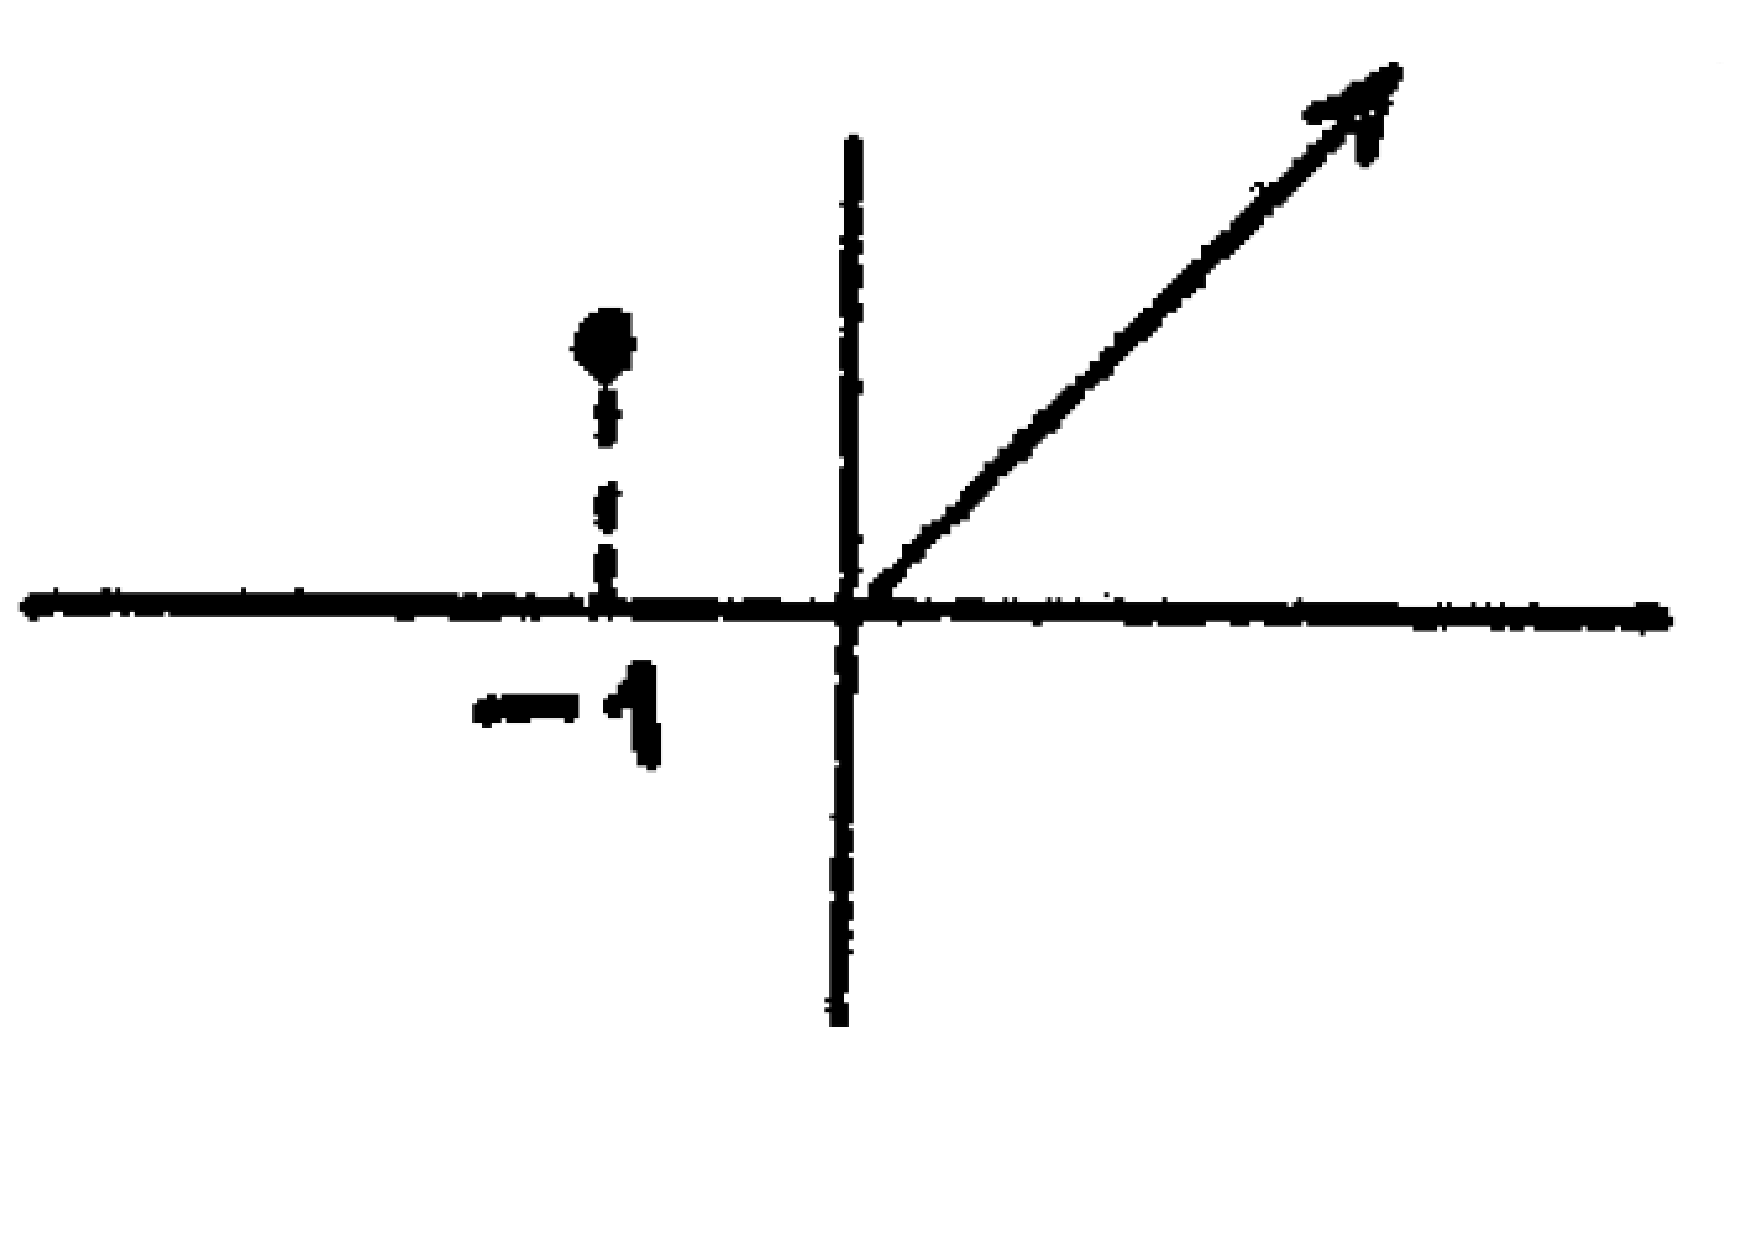
\includegraphics[width=0.45\textwidth]{images/ceyhun-001-samplePage-fig02}
        \label{fig:prob1_6_2}
    \end{minipage} 
    \end{tabular}
    
    
    
    
    